\documentclass{standalone}
\usepackage{tikz}
\usetikzlibrary{arrows.meta, positioning, calc}

\begin{document}
	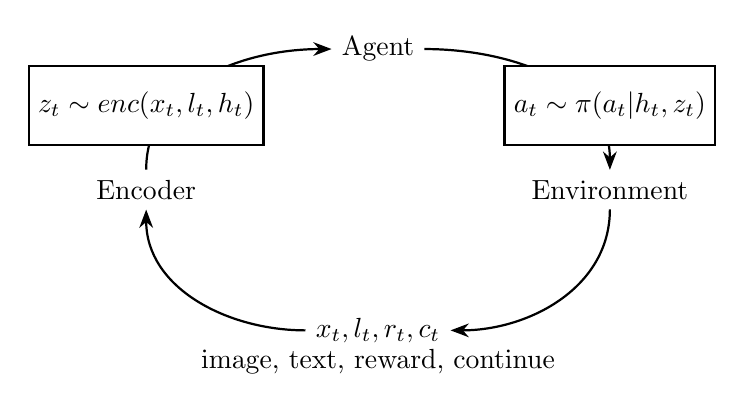
\begin{tikzpicture}[
		node distance=2.5cm,
		thick,
		>=Stealth,
		box/.style={rectangle, draw, align=center, minimum width=2.5cm, minimum height=1cm},
		equation/.style={align=center, font=\normalsize},
		label/.style={font=\normalsize, align=center}
		]
		
		% Main boxes
		\node[label] (encoder) {Encoder}; % $z_t \sim enc(x_t, l_t, h_t)$
		\node[label, right=4cm of encoder] (environment) {Environment}; % $a_t \sim \pi(a_t|h_t, z_t)$
		
		% Agent label at the top
		\node[label, above=1.5cm of $(encoder)!0.5!(environment)$] (agent) {Agent};
		
		% Environment label
		\node[label, below=1.5cm of $(encoder)!0.5!(environment)$] (observation) {$x_t, l_t, r_t, c_t$};
		\node[label, below=1.9cm of $(encoder)!0.5!(environment)$] {image, text, reward, continue};
		
		% Variables at the bottom with labels
		%\coordinate (bottom) at ($(encoder)!0.5!(agent) + (0,-1.8)$);
		%\node[label, at=(bottom)] {$x_t, \; l_t, \; r_t, \; c_t$};
		
		% Individual variable labels
		%\node[label, below=0.4cm of bottom, xshift=-2cm] {image};
		%\node[label, below=0.4cm of bottom, xshift=-0.7cm] {text};
		%\node[label, below=0.4cm of bottom, xshift=0.6cm] {reward};
		%\node[label, below=0.4cm of bottom, xshift=1.9cm] {continue};
		
		% Arrows
		% Top arc from encoder to environment (out is the angle counterclockwise from east)
		\draw[->] (encoder.north) to[out=90, in=180] (agent.west);
		\draw[->] (agent.east) to[out=0, in=90] (environment.north);
		
		% Right arc from environment down to observation
		\draw[->] (environment.south) to[out=-90, in=0] (observation.east);
		
		% Left arc from observation up to encoder
		\draw[->] (observation.west) to[out=180, in=-90] (encoder.south);
		%\draw[->] ($(bottom) + (-2,0)$) to[out=150, in=-150] (encoder.west);
		
		% Labels above boxes
		\node[box, above=0.3cm of encoder, fill=white] {$z_t \sim enc(x_t, l_t, h_t)$};
		\node[box, above=0.3cm of environment, fill=white] {$a_t \sim \pi(a_t|h_t, z_t)$};
		
		
	\end{tikzpicture}
\end{document}